\documentclass[11pt, addpoints, a4paper]{exam}
\usepackage{amsmath, amssymb}
\usepackage{xcolor}
\usepackage{tikz}
\usepackage{enumerate}
\usepackage{graphicx}
\usepackage{tabularx}
\usepackage{algorithm}
\usepackage{algpseudocode}
\usepackage{tikz}
\usepackage{tikz-qtree}
\usepackage{soul}
\usetikzlibrary{graphs}
\tikzset{every tree node/.style={minimum width=2em,draw,circle},
    blank/.style={draw=none},
    edge from parent/.style=
    {draw,edge from parent path={(\tikzparentnode) -- (\tikzchildnode)}},
    level distance=1.2cm}

\newcommand{\red}[1]{\textcolor{red}{#1}}
\newcommand{\blue}[1]{\textcolor{blue}{#1}}

% For inserting code snippets.
\usepackage{listings}
\lstset{
    columns = fixed,
    basewidth = {0.5em},
    breaklines = true,
    backgroundcolor = \color{white},
    keywordstyle = \color[RGB]{40, 40, 255},
    numberstyle = \footnotesize\color{darkgray},
    commentstyle = \ttfamily\color{violet},
    basicstyle = \linespread{1}\small\ttfamily,
    aboveskip = 6pt,
    belowskip = 6pt,
    stringstyle = \ttfamily\color[RGB]{128, 0, 0},
    showstringspaces = false,
    language = {[11]C++},
    escapechar = \@
}
\lstnewenvironment{cpp}[1][]{\lstset{language = {[11]C++}, #1}}{}

\renewcommand{\baselinestretch}{1.15}
\setlength{\parskip}{1.25\baselineskip}

% headers, footers, titles
\newcommand{\CourseName}{CS101 Algorithms and Data Structures}
\newcommand{\HomeworkNO}{5}
\newcommand{\DueDate}{November 8, 2026}

\pagestyle{headandfoot}
\runningheadrule
\runningheader{CS101 Fall26}{Homework \HomeworkNO}{Due on: \DueDate}
\runningfooter{}{\thepage}{}

\title{
    \vspace{25pt}
    \LARGE ShanghaiTech University \\
    \bigskip
    \textbf{\CourseName} \\
    \textbf{Fall 2026}   \\
    \bigskip
    Homework \HomeworkNO
}
\author{}
\date{\large Due date: \DueDate, at 23:59}

% formats of questions, choices, points, etc.
\qformat{\bf\thequestion. (\totalpoints\ points) \thequestiontitle\hfill}
\pointname{'}
% Student version: the source contains no answer key.
% Render the empty solution environments; their height is set with \vspace.
\printanswers

% We frequently use this font.
\newcommand{\ttt}{\texttt}
\newcommand{\bluett}[1]{\textcolor{blue}{\ttt{#1}}}

\begin{document}

\maketitle

\vspace{50pt}

\begin{enumerate}
    \item Please write your solutions in English.
    \item You may discuss the assignment with classmates and AI tools, but you must not directly copy answers or adapt AI-generated contents in any form.
    \item Submit your solutions to Gradescope.
    \item Set your FULL name to your Chinese name and your STUDENT ID correctly in Gradescope account settings.
    \item If you want to submit a handwritten version, scan it clearly. \ttt{CamScanner} is recommended.
    \item We recommend you to write in \LaTeX.
    \item When submitting, match your solutions to the problems correctly.
    \item No late submission will be accepted.
    \item Violations to any of the above may result in zero points.
\end{enumerate}


\begin{questions}
\setlength{\parskip}{0.6\baselineskip}

\newpage
\titledquestion{Multiple Choices}

Each question has \textbf{one or more} correct answer(s). Select all the correct answer(s). For each question, you will get 0 points if you select one or more wrong answers, but you will get 1 point if you select a non-empty subset of the correct answers.

Write your answers in the following table.

% Enter selected choices in the blank table below.

\begin{table}[h]
\centering
\begin{tabular}{|p{1.5cm}|p{1.5cm}|p{1.5cm}|p{1.5cm}|}
        \hline
        (a) & (b) & (c) & (d)  \\
        \hline
          B  &  AB   &  ABC   &     AB     \\[0.7cm]
        \hline
        (e) & (f) & (g) & (h) \\
        \hline
          BC  &  AB   &  ABC   &     AC    \\[0.7cm]
        \hline
    \end{tabular}
\end{table}

\textbf{Note that in this problem, heaps are binary heaps, array-based heap are implemented based on complete binary tree.}

\begin{parts}

\part[3] Which of the following statements about the heap is/are true?
    \begin{choices}
        \choice If a binary tree is a max-heap, then the pre-order traversal of this tree is a descending sequence.
        \choice  For any node A in a heap, the subtree of the tree with root A is still a heap.
        \choice We can sort an array in linear time through heap sort since we can build a heap from an array in O(n) time through Floyd’s method.
        \choice If we pop the minimum element from a binary min-heap and insert the same element back, the heap structure always remains unchanged.
    \end{choices}

\part[3] Which of the following statements about array-based max-heaps is/are true?
    \begin{choices}
        \choice In a zero-indexed heap array, the children of node $i$ are stored at indices $2i+1$ and $2i+2$, whenever these indices exist.
        \choice The array $\langle 50,30,40,10,20,35,37\rangle$ can represent a valid zero-indexed max-heap.
        \choice Replacing the root of a max-heap with any smaller value always preserves the max-heap property.
        \choice Every leaf in a max-heap has a value smaller than every internal node.
    \end{choices}

\part[3] Which of the following statements about heap operations is/are true?
    \begin{choices}
        \choice Building a heap from an arbitrary array using Floyd's bottom-up method takes $O(n)$ time.
        \choice Performing $n$ extract-min operations on a binary min-heap takes $O(n\log n)$ time in the worst case.
        \choice Increasing the key of a node in a max-heap can be performed in $O(\log n)$ time if the node position is known.
        \choice Finding the minimum element in a max-heap always takes $O(1)$ time.
    \end{choices}

\newpage
\part[3] Which of the following statements about binary search trees are true?
    \begin{choices}
        \choice The in-order traversal of a BST containing distinct keys is strictly increasing.
        \choice The pre-order traversal of a BST containing distinct keys uniquely determines the BST.
        \choice Searching for a key in an arbitrary BST with $n$ nodes always takes $O(\log n)$ time.
        \choice The in-order traversal of every BST is a decreasing sequence.
    \end{choices}

\part[3] Which of the following statements about BST search and deletion is/are true?
    \begin{choices}
        \choice Every BST with $n$ nodes has height $O(\log n)$.
        \choice If a node has a right subtree, its in-order successor is the leftmost node in that right subtree.
        \choice If a node has no right subtree, its in-order successor, if it exists, is the lowest ancestor for which the node lies in the left subtree.
        \choice The root of every BST is the median key.
    \end{choices}

\part[3] Which of the following statements about Huffman coding is/are true?
    \begin{choices}
        \choice Huffman's algorithm repeatedly combines the two symbols or subtrees with the smallest frequencies.
        \choice A Huffman code minimizes the weighted average codeword length among all binary prefix codes for the given frequencies.
        \choice Huffman coding always assigns codewords of the same length to all symbols.
        \choice The Huffman coding tree generated for a set of frequencies is always unique.
    \end{choices}

\part[3] Which of the following statements about Huffman trees is/are true?
    \begin{choices}
        \choice Every internal node in a standard binary Huffman tree has exactly two children.
        \choice For $n$ input symbols, Huffman's algorithm performs exactly $n-1$ combine operations.
        \choice A Huffman tree with $n$ different characters has
        exactly $n$ leaves.
        \choice Every Huffman tree must be a complete binary tree.
    \end{choices}

\part[3] Which of the following statements about AVL trees is/are true?
    \begin{choices}
        \choice At every node of an AVL tree, the absolute difference between the heights of its left and right subtrees is at most $1$.
        \choice Every AVL tree is also a complete binary tree.
        \choice Searching for a key in an AVL tree takes $O(\log n)$ time in the worst case.
        \choice For any AVL tree, inserting one key into it may require rotations at every ancestor of the inserted node.
    \end{choices}

\end{parts}


\newpage
\titledquestion{Array Representation of Min-Heap}
We use an array starting at index 0 to store a min complete binary heap, with the root of the heap placed at the index 1.
\begin{parts}


\part[2] Given an array $[0,1,2,8,5,30,10,12,60,7,81,78]$, which represents a min complete binary heap and the entry $1$ is the root at index $1$. Perform the \textbf{pop} operation according to the pop rules discussed in class. After the operation, the array is:
\par\noindent $[0, 2, 5, 8, 7, 30, 10, 12, 60, 78, 81]$

\part[2] Given an array $[0,1,2,8,5,30,10,12,60,7,81,78]$, which represents a min complete binary heap and the entry $1$ is the root at index $1$. Perform the \textbf{push 0} operation according to the pop rules discussed in class. After the operation, the array is:
\par\noindent $[0, 0, 2, 1, 5, 30, 8, 12, 60, 7, 81, 78, 10]$

\part Complete the following C++ skeleton of \textbf{Push} and \textbf{Pop}.
\begin{cpp}
void push(vector<int>& heap, int val) {
    heap.push_back(val); 
    int index = heap.size() - 1;  
    while (index > 1) {
        int parent = ____1____;  
        if (heap[parent] <= heap[index]) {
            break; 
        }
        _______2_______;
        _______3_______; 
    }
}

void pop(vector<int>& heap) {
    heap[1] = ____4____; 
    heap.pop_back(); 
    int index = 1;
    while (index < heap.size()) {
        int left = ____5____;  
        int right = ___6_____;  
        int smallest = index;
        if (left < heap.size() && heap[left] < heap[smallest]) {
            smallest = left;
        }
        if (right < heap.size() && heap[right] < heap[smallest]) {
            smallest = right;
        }
        if (smallest != index) {
            _______7_______;
            _______8_______; 
        } 
        else {
            break; 
        }
    }
}
\end{cpp}
\newpage
\begin{subparts}
    \subpart[2] Choose one of the following statements to fill in the blank 2,3,7,8:
    
        
    \vspace{5pt}
    \begin{checkboxes}
  \choice \begin{lstlisting}[language=C++]
  std::swap(heap[parent], heap[index]); //2
  index = heap.size()-1;   //3
  std::swap(heap[smallest], heap[index]); //7
  index = std::min(left,right); //8
  \end{lstlisting}
  
  \choice \begin{lstlisting}[language=C++]
  index = heap.size()-1;   //2
  std::swap(heap[parent], heap[index]); //3
  index = std::min(left,right); //7
  std::swap(heap[smallest], heap[index]); //8
  \end{lstlisting}

  \CorrectChoice \begin{lstlisting}[language=C++]
  std::swap(heap[parent], heap[index]); //2
  index = parent;   //3
  std::swap(heap[smallest], heap[index]); //7
  index = smallest; //8
  
  \end{lstlisting}
  
  \choice \begin{lstlisting}[language=C++]
  index = parent; //2
  std::swap(heap[parent], heap[index]); //3
  index = smallest; //7
  std::swap(heap[smallest], heap[index]); //8
  
  \end{lstlisting}
\end{checkboxes}

    
    \vspace{15pt}
    \setlength{\parskip}{0.6\baselineskip}
    \subpart[1] Fill in the blank (1):
    \par\noindent index / 2
    
    \vspace{15pt}
    \subpart[1] Fill in the blank (4):
    \par\noindent heap[heap.size() - 1]

    \vspace{15pt}
    \subpart[1] Fill in the blank (5):
    \par\noindent index * 2

    \vspace{15pt}
    \subpart[1] Fill in the blank (6):
    \par\noindent index * 2 + 1
\end{subparts}



\newpage
\part Complete the following C++ skeleton of building a heap through Floyd’s method.
\begin{cpp}
void heapify(vector<int>& heap, int i) {
    int n = heap.size() - 1;
    int left = ...   #dont need answer here
    int right = ...  #dont need answer here
    int smallest = i;        
    if (left <= n && heap[left] < heap[smallest]) {
        smallest = left;
    }
    if (right <= n && heap[right] < heap[smallest]) {
        smallest = right;
    }
    if (smallest != i) {
        _______1_______;
        _______2_______;  
    }
}
void buildHeap(vector<int>& heap) {
    int n = heap.size() - 1;
    for (int i = _______3_______) #Only necessary iterations, not 1...n
    {
        heapify(heap, i);  
    }
}
\end{cpp}
\begin{subparts}

    \vspace{15pt}
    \setlength{\parskip}{0.6\baselineskip}
    \subpart[1] Fill in the blank (1):
    \par\noindent std::swap(heap[i], heap[smallest])
    
    \vspace{15pt}
    \subpart[1] Fill in the blank (2):
    \par\noindent heapify(heap, smallest)

    \vspace{15pt}
    \subpart[1] Fill in the blank (3):
    \par\noindent n / 2; i >= 1; i--

\end{subparts}

\newpage
\part[3] Assume that all keys are distinct and that the input keys are generated in a uniformly random order. The heap is obtained by inserting the first $n$ keys in this order, and the new entry is the $(n+1)$-st key.

Write down the \textbf{average} time complexity of the following operations in a min complete binary heap of size $n$: (don't need to prove; use $\Theta$):
\begin{itemize}
    \item[1.] Access the root.
    \item[2.] Pop the root.
    \item[3.] Build a heap by Floyd’s Method.
    \item[4.] Merge two binary heaps of size $n$.
    \item[5.] Push a randomly generated entry.
    \item[6.] Push an entry smaller the root of the heap.
\end{itemize}
\begin{solution}
\begin{enumerate}
    \item[1.] $\Theta(1)$
    \item[2.] $\Theta(\log n)$
    \item[3.] $\Theta(n)$
    \item[4.] $\Theta(n)$
    \item[5.] $\Theta(1)$
    \item[6.] $\Theta(\log n)$
\end{enumerate}
\end{solution}
\end{parts}


\newpage
\titledquestion{Min-Max-Heap}
\setlength{\parskip}{0pt}
A \textit{min-max-heap} is a data structure which supports both \texttt{popMin()} and \texttt{popMax()} operations in $O(\log n)$ time. A min-max-heap is still a complete binary tree, but it has the following properties:

\begin{itemize}
    \item For every element at even depth (on \textcolor{blue}{min-level}), it is smaller than its parent (if existing) and greater than its grandparent (the parent node of its parent node, if existing). In short: \textbf{\ttt{x\(<\)parent(x)} and \ttt{x\(>\)grandparent(x)} for \ttt{x} on min-level}.
    \item For every element at odd depth (on \textcolor{red}{max-level}), it is greater than its parent and smaller than its grandparent(if existing). In short: \textbf{\ttt{x\(>\)parent(x)} and \ttt{x\(<\)grandparent(x)} for \ttt{x} on max-level}.
\end{itemize} 

You can assume that all nodes are distinct and there are always more than one nodes in this question. Please see the following example min-max-heap, as shown in the figure below:

\noindent\begin{minipage}{\linewidth}
\centering
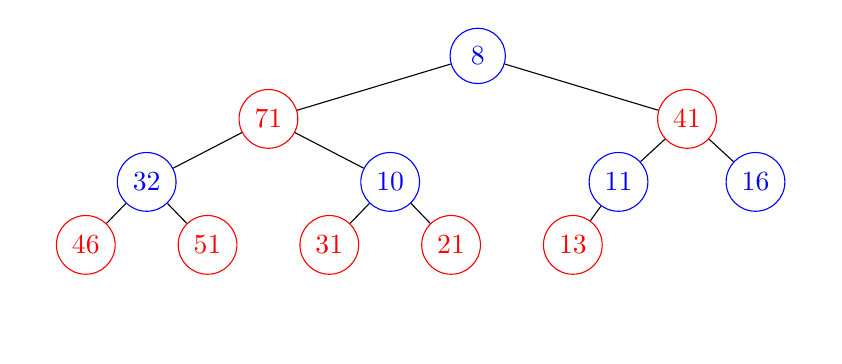
\begin{tikzpicture}[level distance=0.8cm]
\Tree
[.\node[blue]{8};
    [.\node[red]{71};
        \edge[]; [.\node[blue]{32};
            \edge[]; [.\node[red]{46};
                \edge[blank]; \node[blank]{};
                \edge[blank]; \node[blank]{};
            ]
            \edge[]; [. \node[red]{51};
                \edge[blank]; \node[blank]{};
                \edge[blank]; \node[blank]{};
            ]
        ]
        \edge[]; [.\node[blue]{10};
            \edge[]; [.\node[red]{31};
                \edge[blank]; \node[blank]{};
                \edge[blank]; \node[blank]{};
            ]
            \edge[]; [.\node[red]{21};
                \edge[blank]; \node[blank]{};
                \edge[blank]; \node[blank]{};
            ]
        ]
    ]
    [.\node[red]{41};
        \edge[]; [.\node[blue]{11};
            \edge[]; [.\node[red]{13};
                \edge[blank]; \node[blank]{};
                \edge[blank]; \node[blank]{};
            ]
            \edge[blank]; \node[blank]{};
        ]
        \edge[]; [.\node[blue]{16};
            \edge[blank]; \node[blank]{};
            \edge[blank]; \node[blank]{};
        ]
    ]
]
\end{tikzpicture}
\end{minipage}
\vspace{-0.3in}

\begin{parts}
\part[4] \textbf{Let's See What's New about Min-Max-Heap}\par
For each of the following statements about min-max-heap, please judge whether it is true or false. Tick (\(\surd\)) the correct answer. Assume the parent and the children of the node \ttt{x} all exist.
\begin{subparts}
\setlength{\parskip}{0pt}
    
    \subpart \label{a} If \ttt{x} is on min-level, then its parent and children are also on min-level. 
    \par\nobreak\hfill\mbox{\begin{oneparcheckboxes}
        \choice True
        \CorrectChoice False
    \end{oneparcheckboxes}}
    
    \subpart If \ttt{x} is on min-level, then \ttt{x} is less than both of its children.
    \par\nobreak\hfill\mbox{\begin{oneparcheckboxes}
        \CorrectChoice True
        \choice False
    \end{oneparcheckboxes}}
    
    \subpart If \ttt{x} is on max-level and \ttt{x} is a strict ancestor of \ttt{y}, then \ttt{x\(<\)y}.
    \par\nobreak\hfill\mbox{\begin{oneparcheckboxes}
        \choice True
        \CorrectChoice False
    \end{oneparcheckboxes}}
    
    \subpart The minimum is on min-level and the maximum is on max-level.
    \par\nobreak\hfill\mbox{\begin{oneparcheckboxes}
        \CorrectChoice True
        \choice False
    \end{oneparcheckboxes}}
\end{subparts}



\part[4] \textbf{Where is Min and Max?}\par
How do we search the minimum element, the maximum element and the second-smallest element in a min-max-heap with \(n(n \geq 7) \) elements? What is their time complexity?
\begin{solution}
    The minimum element is at the root and the maximum element is at one of the root's children.

    The second-smallest element is at one of the four nodes at depth 2.

    The time complexity of searching them is all $O(1)$.
\end{solution}


\newpage
\setlength{\parskip}{0.6\baselineskip}
\part \textbf{Percolate it Up!}\par
Similar to a common heap we learned in the lectures, the new element is inserted at the first available leaf and we will maintain the heap property along the path from this leaf node to the root node, which is called a \textbf{percolation-up}. The c++ styled code of \textbf{percolation-up in a min-max-heap} is given below(assume function parent() and grandparent() have been implemented): 

\begin{lstlisting}[language=C++]
void percolateUp(int i) {
    // Assume parent(i) exists.

    if (isMaxLevel(i)) {
        if (/* [1] */) {
            while (grandparent(i) != -1 &&
                   /* [2] */) {
                int g = grandparent(i);
                std::swap(H[i], H[g]);
                i = g;
            }
        } else {
            int p = parent(i);
            std::swap(H[i], H[p]);
            i = p;

            while (grandparent(i) != -1 &&
                   /* [3] */) {
                int g = grandparent(i);
                std::swap(H[i], H[g]);
                i = g;
            }
        }
    } else {
        // This case is omitted.
    }
}
\end{lstlisting}

    
\begin{subparts}
    \subpart[2] Choose one of the following statements to fill in the blank (1):
    
    \vspace{5pt}
    \begin{checkboxes}
        \choice \ttt{H[i]\(<\)H[parent(i)]}
        \choice \ttt{H[i]\(<\)H[grandparent(i)]}
        \CorrectChoice \ttt{H[i]\(>\)H[parent(i)]}
        \choice \ttt{H[i]\(>\)H[grandparent(i)]}
    \end{checkboxes}
    
    \vspace{15pt}
    \setlength{\parskip}{0.6\baselineskip}
    \subpart[1] Fill in the blank (2):
    \par\noindent H[i] > H[grandparent(i)]
    
    \vspace{15pt}
    \subpart[1] Fill in the blank (3):
    \par\noindent H[i] < H[grandparent(i)]
\end{subparts}


\newpage


\part[3] \textbf{Percolate it Down?}\par
Similarly, when popping a node off the min-max-heap, we move the last leaf node to the \textit{hole} and percolate it down. However, the \textbf{percolation-down} procedure in a min-max-heap is a bit more complicated.

In this question, just consider you are popping the minimum off the example min-max-heap shown above (it is shown again below for your convenience). Please draw the min-max-heap after this \ttt{popMin()}.

Just draw the heap after \ttt{popMin()} directly, you don't need to show the intermediate steps.

\vspace{20pt}
\noindent\begin{minipage}{\linewidth}
\centering
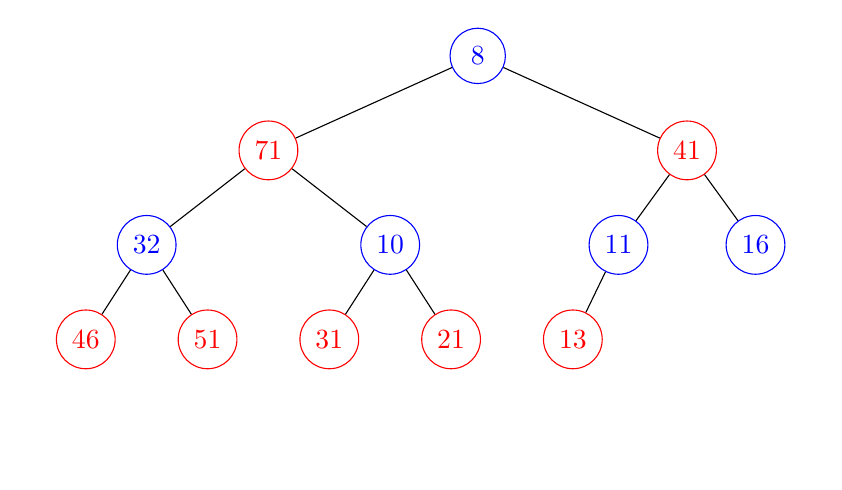
\begin{tikzpicture}
\Tree
[.\node[blue]{8};
    [.\node[red]{71};
        \edge[]; [.\node[blue]{32};
            \edge[]; [.\node[red]{46};
                \edge[blank]; \node[blank]{};
                \edge[blank]; \node[blank]{};
            ]
            \edge[]; [. \node[red]{51};
                \edge[blank]; \node[blank]{};
                \edge[blank]; \node[blank]{};
            ]
        ]
        \edge[]; [.\node[blue]{10};
            \edge[]; [.\node[red]{31};
                \edge[blank]; \node[blank]{};
                \edge[blank]; \node[blank]{};
            ]
            \edge[]; [.\node[red]{21};
                \edge[blank]; \node[blank]{};
                \edge[blank]; \node[blank]{};
            ]
        ]
    ]
    [.\node[red]{41};
        \edge[]; [.\node[blue]{11};
            \edge[]; [.\node[red]{13};
                \edge[blank]; \node[blank]{};
                \edge[blank]; \node[blank]{};
            ]
            \edge[blank]; \node[blank]{};
        ]
        \edge[]; [.\node[blue]{16};
            \edge[blank]; \node[blank]{};
            \edge[blank]; \node[blank]{};
        ]
    ]
]
\end{tikzpicture}
\end{minipage}

\begin{solution}

\begin{minipage}{\linewidth}
\centering
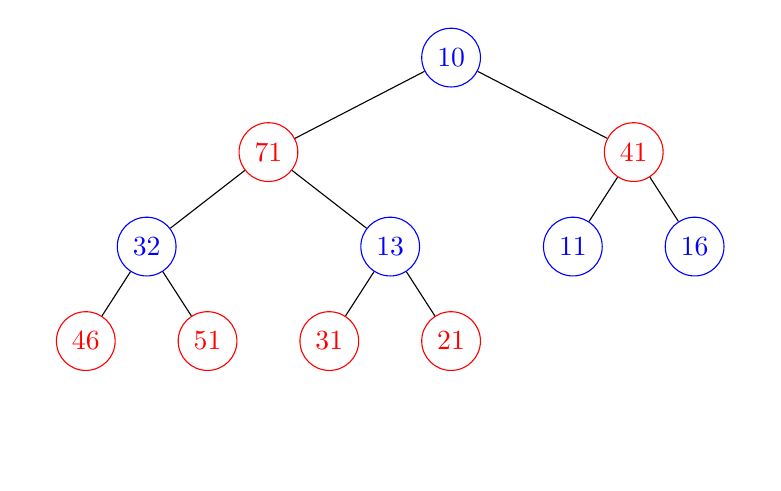
\begin{tikzpicture}
\Tree
[.\node[blue]{10};
    [.\node[red]{71};
        \edge[]; [.\node[blue]{32};
            \edge[]; [.\node[red]{46};
                \edge[blank]; \node[blank]{};
                \edge[blank]; \node[blank]{};
            ]
            \edge[]; [.\node[red]{51};
                \edge[blank]; \node[blank]{};
                \edge[blank]; \node[blank]{};
            ]
        ]
        \edge[]; [.\node[blue]{13};
            \edge[]; [.\node[red]{31};
                \edge[blank]; \node[blank]{};
                \edge[blank]; \node[blank]{};
            ]
            \edge[]; [.\node[red]{21};
                \edge[blank]; \node[blank]{};
                \edge[blank]; \node[blank]{};
            ]
        ]
    ]
    [.\node[red]{41};
        \edge[]; [.\node[blue]{11};
            \edge[blank]; \node[blank]{};
            \edge[blank]; \node[blank]{};
        ]
        \edge[]; [.\node[blue]{16};
            \edge[blank]; \node[blank]{};
            \edge[blank]; \node[blank]{};
        ]
    ]
]
\end{tikzpicture}
\end{minipage}
\end{solution}
\newpage
\part[5]A \textit{deletable heap} supports deletion of an arbitrary element by using
\textbf{lazy deletion}. Instead of immediately removing an element from the
heap, we mark its unique identifier as deleted. Whenever an element is about
to be returned from the heap, all deleted elements at the top are removed.

Instead of storing a min-max-heap directly, we maintain two deletable heaps:

\begin{itemize}
    \item a min-heap \texttt{minHeap};
    \item a max-heap \texttt{maxHeap}.
\end{itemize}

Every inserted element is stored in both heaps. Both heaps contain the same
pair \texttt{(key, id)}. The set \texttt{Deleted} stores the identifiers of
logically deleted elements.
Complete the following c++ code.
\begin{lstlisting}[language=C++]
struct Entry {
    int key;
    int id;
};
struct MinCompare {
    bool operator()(const Entry& a, const Entry& b) const {
        if (a.key != b.key)
            return a.key > b.key;
        return a.id > b.id;
    }
};
struct MaxCompare {
    bool operator()(const Entry& a, const Entry& b) const {
        if (a.key != b.key)
            return a.key < b.key;
        return a.id < b.id;
    }
};

std::priority_queue<Entry,std::vector<Entry>,MinCompare> minHeap;
std::priority_queue<Entry,std::vector<Entry>,MaxCompare> maxHeap;
std::unordered_set<int> Deleted;
int nextID = 0;

void cleanMin() {
    while (!minHeap.empty() && Deleted.count(minHeap.top().id) > 0) {
        minHeap.pop();
    }
}
void cleanMax() {
    while (!maxHeap.empty() && Deleted.count(maxHeap.top().id) > 0) {
        maxHeap.pop();
    }
}

\end{lstlisting}
\newpage
\begin{lstlisting}[language=C++]
int insert(int key) {
    int id = nextID++;
    /* [1] */
    /* [2] */
    return id;
}
void erase(int id) {
    Deleted.insert(id);
}
Entry findMin() {
    cleanMin();
    return minHeap.top();
}
Entry findMax() {
    cleanMax();
    return maxHeap.top();
}
Entry popMin() {
    cleanMin();
    Entry x = /* [3] */
    /* [4] */
    Deleted.insert(x.id);
    return x;
}
Entry popMax() {
    cleanMax();
    Entry x = /* [5] */
    /* [6] */
    Deleted.insert(x.id);
    return x;
}
\end{lstlisting}

\begin{solution}
\begin{enumerate}
    \item[[1]] minHeap.push({key, id});
    \item[[2]] maxHeap.push({key, id});
    \item[[3]] minHeap.top();
    \item[[4]] minHeap.pop();
    \item[[5]] maxHeap.top();
    \item[[6]] maxHeap.pop();
\end{enumerate}
\end{solution}
\end{parts}


\newpage
\titledquestion{Find the median}

Given a binary search tree storing n integers (assuming n is odd), design an algorithm to query the median of all integers in the tree.

\begin{parts}
    \part[6] Fill in the blank.
    \begin{cpp}[basicstyle=\linespread{1}\fontsize{9}{10}\selectfont\ttfamily]
// Binary Search Tree Node
struct Node {
    int val;
    Node* left;
    Node* right;
    int size;
    Node(int x) : val(x), left(nullptr), right(nullptr), size(1) {}
};
// Binary Search Tree
// Fill only the blanks; the other omitted code is irrelevant.
class BST {
private:
    Node* root;
    void update(Node* node) {
        if (!node) return;
        int left_size = node->left ? node->left->size : 0;
        int right_size = node->right ? node->right->size : 0;
        node->size = left_size + right_size + 1;
    }
    Node* insert(Node* node, int val) {
        if (!node) {
            return new Node(val);
        }
        if (val < node->val) {
            node->left = insert(node->left, val);
        } else if (val > node->val) {
            node->right = insert(node->right, val);
        }
        update(node);
        return node;
    }
    int find(Node* node, int k) {
        if (!node) return -1;
        int left_size = node->left ? node->left->size : 0;
        if (k <= left_size) {
            return find(node->left, k);
        } else if (k == left_size + 1) {
            return node->val;
        } else {
            return find(node->right, k - left_size - 1);
        }
    }
...
Public:
    // The function for finding the median
    int findMedian() {
        if (!root) {
            return -1;
        }
        int k = (root->size + 1) / 2;
        return find(root, k);
    }
...
}
    \end{cpp}

    \part[2] Suppose a total of $q$ median queries and a total of $k$ insert or delete operations are executed, and $n \leq k, q$, then the time complexity of this algorithm \textbf{in average} is $O((k + q) \log n)$.
\end{parts}


\newpage
\tikzset{
  level 1/.style={level distance=50pt, sibling distance=100pt},
  level 2/.style={level distance=50pt, sibling distance=70pt},
  level 3/.style={level distance=50pt, sibling distance=50pt},
  level 4/.style={level distance=60pt, sibling distance=30pt},
  level 5/.style={level distance=60pt, sibling distance=20pt},
}

\titledquestion{Huffman Coding}

Consider the document
\[
S=\texttt{AAAABBBCCDAAAAEEEEE}.
\]

Each original character requires $8$ bits.

For Huffman coding, any valid optimal code is accepted. The Huffman tree is
stored using the following format:

\begin{itemize}
    \item An internal node requires $1$ bit.
    \item A leaf node requires $1+8$ bits: one marker bit and the
    8-bit ASCII code of the character.
\end{itemize}

\begin{parts}

    \part[3] Construct one valid optimal Huffman code for the characters in
    $S$. Give the codeword of every character and calculate the number of bits
    required to encode $S$, excluding the tree header.

    \begin{solution}
    
    A: 8 times;

    B: 3 times;

    C: 2 times;

    D: 1 time;

    E: 5 times.

    A: 0

    E: 10

    B: 110

    C: 1111

    D: 1110

    $$
    \text{Bits} = 8 \times 1 + 5 \times 2 + 3 \times 3 + 2 \times 4 + 1 \times 4 = 39 \text{ bits}
    $$

    \end{solution}

    \part[2] Calculate the number of bits required to store the Huffman tree
    and the total size of the compressed document.

    \begin{solution}
    
    $$
    \text{Tree header size} = 4 \times 1 + 5 \times (1+8) = 49 \text{ bits} 
    $$

    $$
    \text{Total size} = 39 + 49 = 88 \text{ bits}
    $$
    \end{solution}

    \part[2] Apply run-length encoding(RLE) to $S$, where each maximal same letters are
    represented as a token $(\text{character},\text{length})$.

    Give the resulting token sequence and the frequency of every distinct token.

    \begin{solution}
    
    The token sequence is

    $$
    [(\text{A}, 4), (\text{B}, 3), (\text{C}, 2), (\text{D}, 1), (\text{A}, 4), (\text{E}, 5)]
    $$

    And the frequency of every distinct token is

    (A, 4): 2 times;

    (B, 3): 1 time;

    (C, 2): 1 time;

    (D, 1): 1 time;

    (E, 5): 1 time.
    \end{solution}

    \part[3] Construct one valid optimal Huffman code for the RLE tokens.
    Give the codeword of every distinct token and calculate the number of bits
    required to encode the token sequence, excluding the token-tree header.

    \begin{solution}
    
    (B, 3): 00

    (C, 2): 01

    (A, 4): 10

    (D, 1): 110

    (E, 5): 111

    $$
    \text{Bits} = 2 \times 2 + 1 \times 2 + 1 \times 2 + 1 \times 3 + 1 \times 3 = 14 \text{ bits}
    $$
    \end{solution}

    \part[3] For the RLE Huffman tree, a leaf token requires
    \[
    1+8+4 \ bits
    \]
    one marker bit, the 8-bit ASCII code of the character, and a
    4-bit representation of the run length.

    Calculate the total size of the RLE-compressed document, including the
    token-tree header. Compare it with the result from part (b).Explain why RLE does not always improve
    compression after the tree header is included.

    \begin{solution}
    
    $$
    \text{Tree header size of RLE Huffman tree} = 4 + 5 \times (1+8+4) = 69 \text{ bits}
    $$

    $$
    \text{Total size of RLE Huffman Tree} = 14 + 69 = 83 \text{ bits}
    $$

    Although the pure coding data has been significantly reduced from $39 \text{ bits}$ to $14 \text{ bits}$, the total size has only decreased by $5 \text{ bits}$ due to the increase in tree header from $49 \text{ bits}$ to $69 \text{ bits}$.

    Each leaf node of the RLE Huffman tree not only needs to store the character itself ($8$ bits), but also needs to store the binary digits of the run-length length ($4$ bits here) additionally, which increases the description overhead of each distinct item in the tree header.

    In addition, when the character repetition is not high, the additional overhead caused by tree head expansion will directly offset or even exceed the space saved by the encoding of the data body.
    \end{solution}

\end{parts}


\newpage
\end{questions}


\end{document}
